\documentclass{beamer}
\usepackage{amsmath}
\usepackage[english]{babel} %set language; note: after changing this, you need to delete all auxiliary files to recompile
\usepackage[utf8]{inputenc} %define file encoding; latin1 is the other often used option
\usepackage{csquotes} % provides context sensitive quotation facilities
\usepackage{graphicx} %allows for inserting figures
\usepackage{booktabs} % for table formatting without vertical lines
\usepackage{textcomp} % allow for example using the Euro sign with \texteuro
\usepackage{stackengine}
\usepackage{wasysym}
\usepackage{tikzsymbols}
\usepackage{textcomp}
% ELIMINAR COMANDOS DE NAVEGACION%%%%%%%%%%%
\setbeamertemplate{navigation symbols}

%\newcommand{\bubblethis}[2]{
 %       \tikz[remember picture,baseline]{\node[anchor=base,inner sep=0,outer sep=0]%
 %       (#1) {\underline{#1}};\node[overlay,cloud callout,callout relative pointer={(0.2cm,-0.7cm)},%
 %       aspect=2.5,fill=yellow!90] at ($(#1.north)+(-0.5cm,1.6cm)$) {#2};}%
 %   }%
%\tikzset{face/.style={shape=circle,minimum size=4ex,shading=radial,outer sep=0pt,
 %       inner color=white!50!yellow,outer color= yellow!70!orange}}

%% Some commands to make the code easier
\newcommand{\emoticon}[1][]{%
  \node[face,#1] (emoticon) {};
  %% The eyes are fixed.
  \draw[fill=white] (-1ex,0ex) ..controls (-0.5ex,0.2ex)and(0.5ex,0.2ex)..
        (1ex,0.0ex) ..controls ( 1.5ex,1.5ex)and( 0.2ex,1.7ex)..
        (0ex,0.4ex) ..controls (-0.2ex,1.7ex)and(-1.5ex,1.5ex)..
        (-1ex,0ex)--cycle;}
\newcommand{\pupils}{
  %% standard pupils
  \fill[shift={(0.5ex,0.5ex)},rotate=80] 
       (0,0) ellipse (0.3ex and 0.15ex);
  \fill[shift={(-0.5ex,0.5ex)},rotate=100] 
       (0,0) ellipse (0.3ex and 0.15ex);}

\newcommand{\emoticonname}[1]{
  \node[below=1ex of emoticon,font=\footnotesize,
        minimum width=4cm]{#1};}
\usepackage{scalerel}
\usetikzlibrary{positioning}
\usepackage{xcolor,amssymb}
\newcommand\dangersignb[1][2ex]{%
  \scaleto{\stackengine{0.3pt}{\scalebox{1.1}[.9]{%
  \color{red}$\blacktriangle$}}{\tiny\bfseries !}{O}{c}{F}{F}{L}}{#1}%
}
\newcommand\dangersignw[1][2ex]{%
  \scaleto{\stackengine{0.3pt}{\scalebox{1.1}[.9]{%
  \color{red}$\blacktriangle$}}{\color{white}\tiny\bfseries !}{O}{c}{F}{F}{L}}{#1}%
}
\usepackage{fontawesome} % Social Icons
\usepackage{epstopdf} % allow embedding eps-figures
\usepackage{tikz} % allows drawing figures
\usepackage{amsmath,amssymb,amsthm} %advanced math facilities
\usepackage{lmodern} %uses font that support italic and bold at the same time

\usepackage{tikz}

\usepackage{tcolorbox}


\usefonttheme[onlymath]{serif} %set math font to serif ones

\definecolor{beamerblue}{rgb}{0.2,0.2,0.7} %define beamerblue color for later use

%%% defines highlight command to set text blue
\newcommand{\highlight}[1]{{\color{blue}{#1}}}


%%%%%%% commands defining backup slides so that frame numbering is correct

\newcommand{\backupbegin}{
   \newcounter{framenumberappendix}
   \setcounter{framenumberappendix}{\value{framenumber}}
}
\newcommand{\backupend}{
   \addtocounter{framenumberappendix}{-\value{framenumber}}
   \addtocounter{framenumber}{\value{framenumberappendix}}
}

%%%% end of defining backup slides

%Specify figure caption, see also http://tex.stackexchange.com/questions/155738/caption-package-not-working-with-beamer
\setbeamertemplate{caption}{\insertcaption} %redefines caption to remove label "Figure".
%\setbeamerfont{caption}{size=\scriptsize,shape=\itshape,series=\bfseries} %sets figure  caption bold and italic and makes it smaller

\newtcolorbox{boxA}{
    fontupper = \bf,
    boxrule = 1.5pt,
    colframe = black % frame color
}

\usetheme{Boadilla}

% --------------------
% Overall information
% --------------------
\title[Economía I]{Economía I \vspace{4mm}
\\ Magistral 10: Equilibrio de mercado}
\date{}
\author[Riottini]{Franco Riottini}
\vspace{0.4cm}
\institute[]{Universidad de San Andrés} 

\begin{document}

\begin{frame}
\titlepage
\centering

\includegraphics[scale=0.2]{../Figures/logoUDESA.jpg} 
\end{frame} 

\begin{frame}
\frametitle{Motivación: El precio de TurboMan}
\centering
\href{https://www.youtube.com/watch?v=UIBRtxVG_LE&list=PL1Sd7Ozmz5CcoC_5lrL0pLKYXXLOLUhd2&index=12}{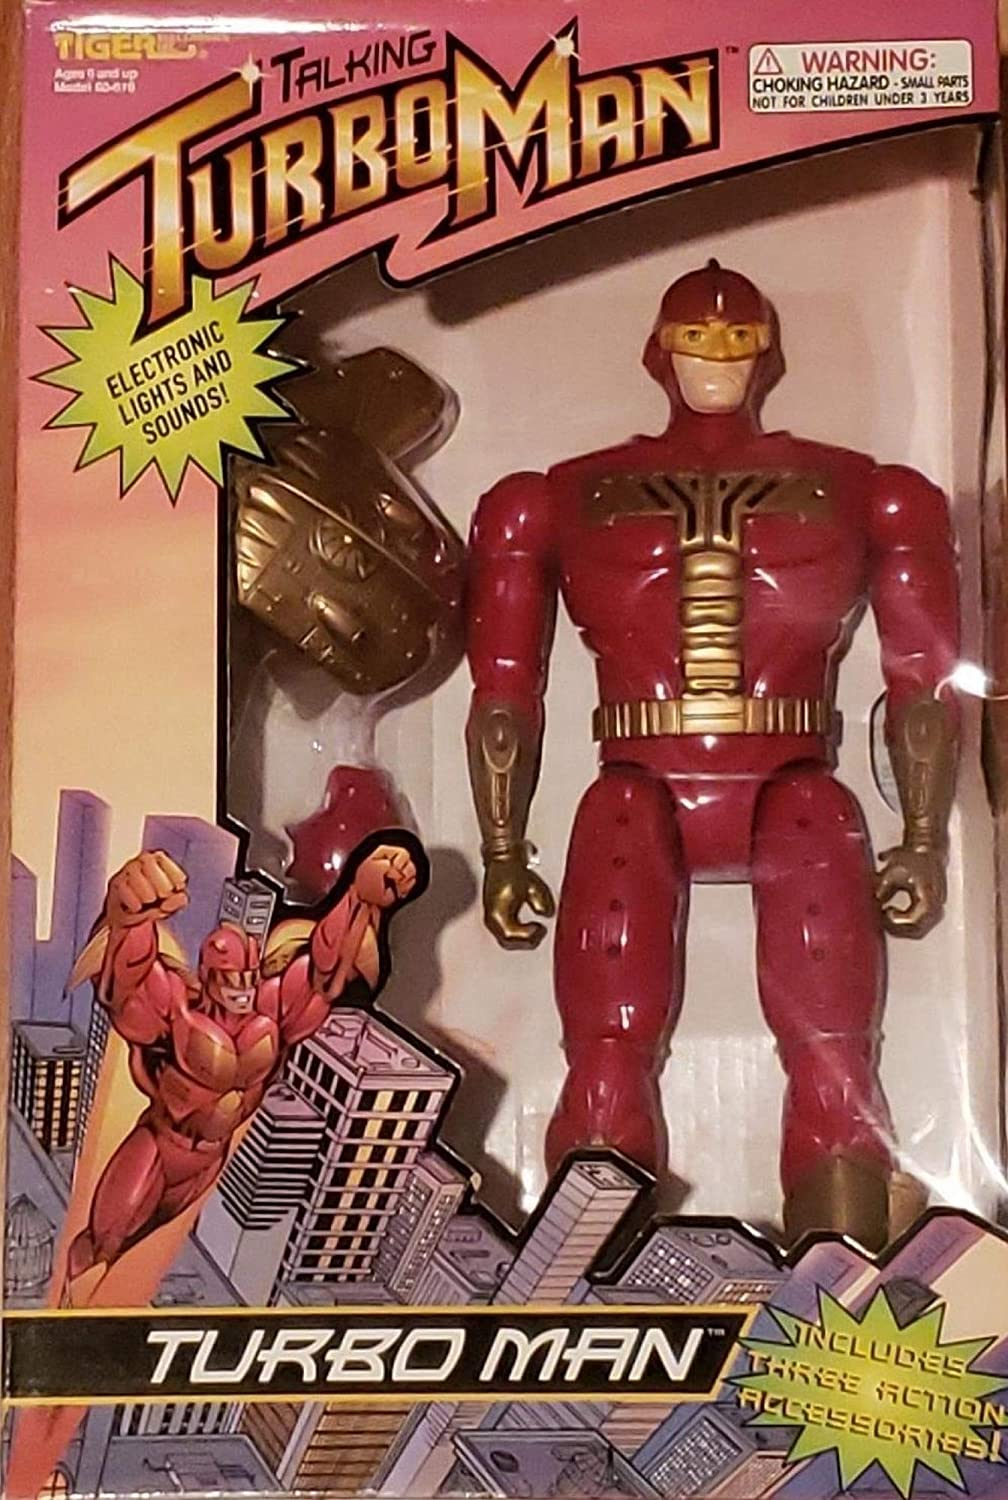
\includegraphics[scale=0.1]{../Figures/Tema_04.01_Turboman.jpg}}
\end{frame}

\begin{frame}
\frametitle{Motivación: El precio del petroleo}
\centering
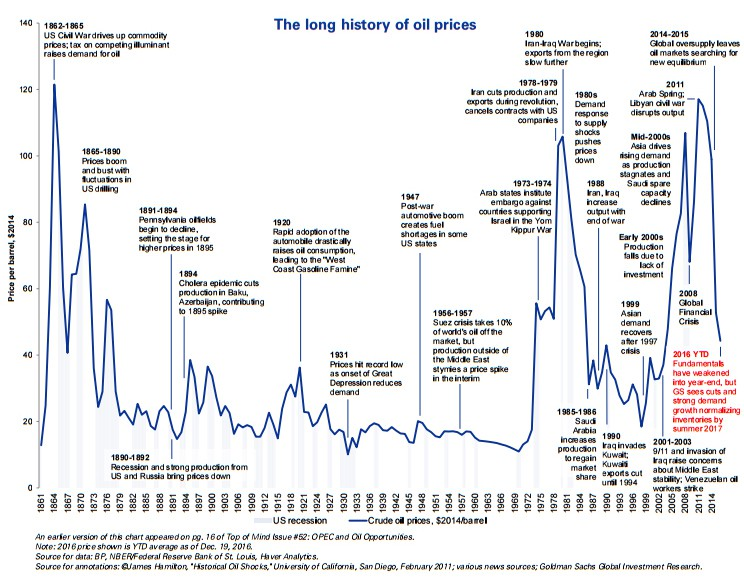
\includegraphics[scale=0.35]{../Figures/Tema_04.01_new.jpg}
\end{frame} 

\begin{frame}
\frametitle{Al precio lo determinan la demanda y la oferta}
\begin{itemize}
    \item Por un lado, tenemos la curva de demanda
    \begin{itemize}
        \item Muestra la cantidad total que los consumidores están dispuestos a comprar a cualquier precio dado
        \item Representa la disposición a pagar (willingness to pay) dinero por los productos que compran
    \end{itemize}
    \vspace{2mm}
    \item Por otro lado, tenemos la curva de oferta
    \begin{itemize}
        \item Muestra la cantidad total que las empresas producirían a cualquier precio dado
        \item Representa la disposición a aceptar (willingness to accept) dinero por los productos que venden
        \item Refleja entonces los distintos precios de reserva de estos vendedores
        \end{itemize}
\end{itemize}
\end{frame}

\begin{frame}
\frametitle{La curva de demanda}
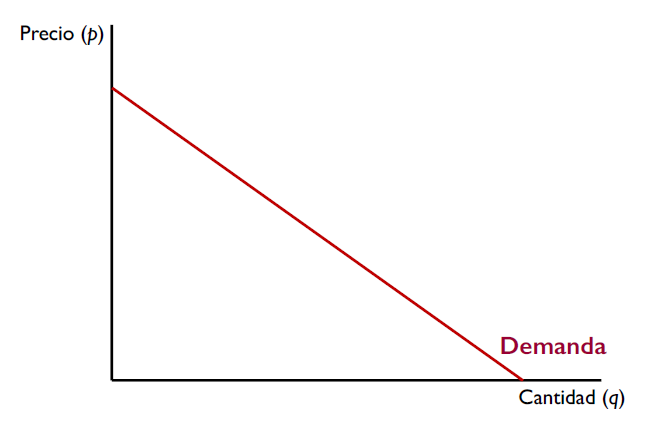
\includegraphics[scale=0.6]{../Figures/Tema_07.1_curvadeldemanda.png}
%Figura 10.4
\end{frame}

\begin{frame}
\frametitle{Desplazamientos sobre la curva de demanda}
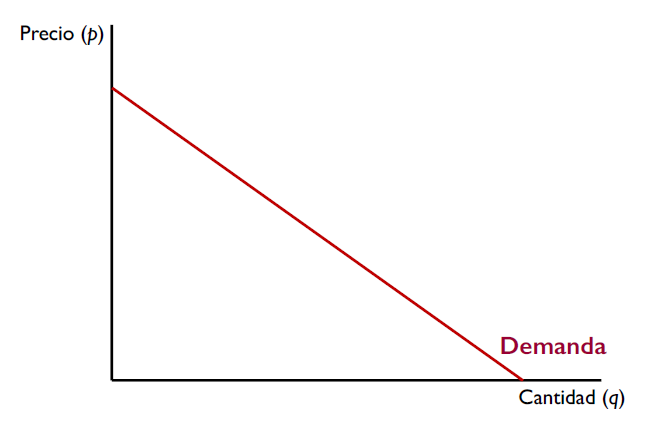
\includegraphics[scale=0.6]{../Figures/Tema_07.1_curvadeldemanda.png}
%Figura 10.5
\end{frame}

\begin{frame}
\frametitle{Desplazamientos de la curva de demanda}
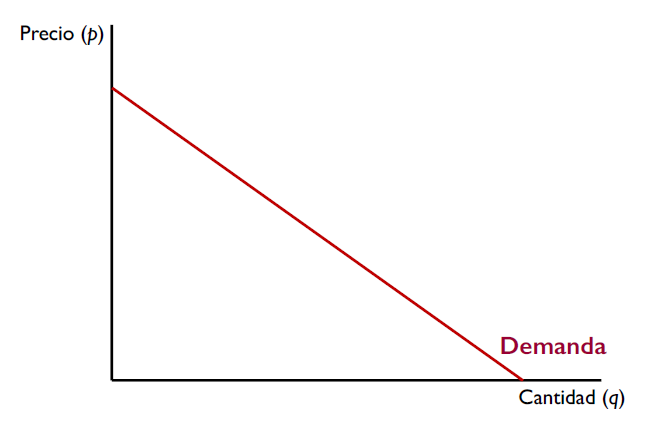
\includegraphics[scale=0.6]{../Figures/Tema_07.1_curvadeldemanda.png}
%Figura 10.6
\end{frame}

\begin{frame}
\frametitle{¿Qué factores afectan la función de demanda?}
\begin{itemize}
    \item Ingresos %Ej Aumenta el ingreso slide con link a Figura 10.6 panel a  
    \item Precio de bienes que son sustitutos %link a Figura
    \item Precio de bienes que son complementarios %link a Figura
    \item Número de compradores %link a Figura
    \item Gustos y preferencias %link a Figura
    \item Expectativas %link a Figura
    \item Influencias especiales %link a Figura
\end{itemize}
\end{frame}
% La idea de esta slide es que muestre un ejemplo de cada factor, que vean que la demanda se desplaza con todos ellos

%%%%%%%%%% SEPARAR CAPITULO 
%%%%%%%%%%%%%%%%%%%%%%%%%%%%%%%%%%%%%%%%%%%%%%%%%%%%%%%%%
%\title[Principios de Economía]{Principios de Economía %\vspace{4mm}
%\\ Capítulo 14: Construyendo la oferta}
%\date{}
%\vspace{0.4cm}
%\institute[]{Introduzca su nombre aquí} 

%%%%%%%%%%%%%%%%%%%%%%%%%%%%%%%%%%%%%%%%%%%%%%%%%%%%%%%%%%%% 

%\begin{document}

%\begin{frame}
%\titlepage
%\centering
%
\includegraphics[scale=0.2]{../Figures/logoUDESA.jpg} 
%\end{frame} 
%%%%%%%%%%%%%%%%%%%%%%%%%%%%%%%%%%%%%%%%%%%%%%%%%%%%%%%%

\begin{frame}
\frametitle{La curva de oferta}
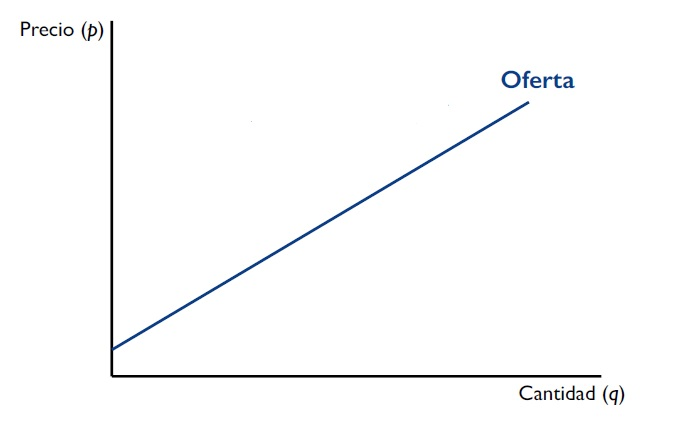
\includegraphics[scale=0.6]{../Figures/Tema_07.2_curvadeoferta.jpg}
%Figura 14.2 pero modificada para que no haya dos puntos, que este solo el punto A
\end{frame}


\begin{frame}
\frametitle{Desplazamientos sobre la curva de oferta}
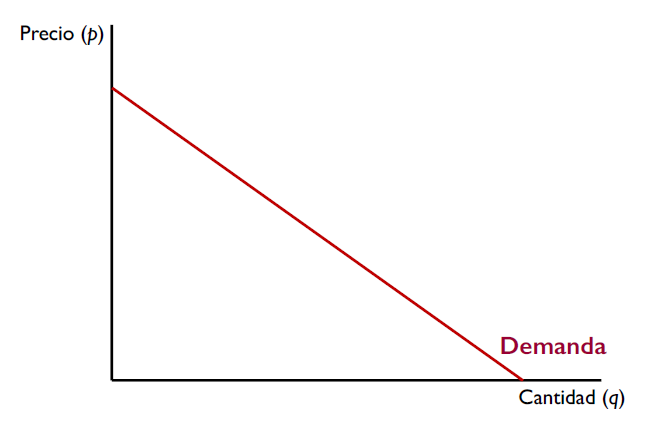
\includegraphics[scale=0.6]{../Figures/Tema_07.1_curvadeldemanda.png}
%Figura 14.2
\end{frame}

\begin{frame}
\frametitle{Desplazamientos de la curva de demanda}
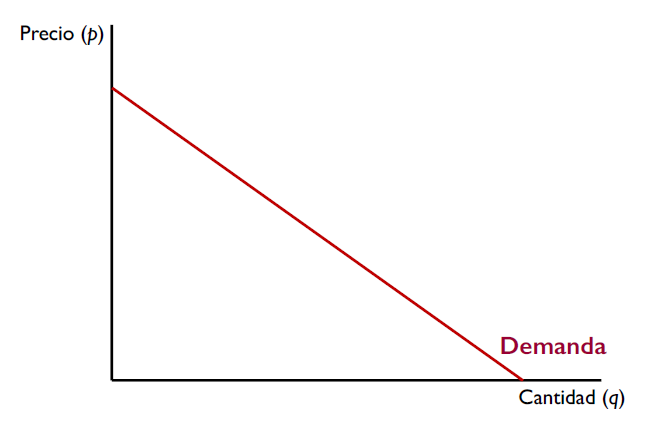
\includegraphics[scale=0.6]{../Figures/Tema_07.1_curvadeldemanda.png}
%Figura 10.
\end{frame}

\begin{frame}
\frametitle{¿Qué factores afectan la función de oferta?}
\begin{itemize}
    \item Precio de los insumos %Ej Aumenta el precio de un insumo slide con link a Figura 14.3 panel b  
    \item Tecnología %Ej
    \item Precios de bienes relacionados %Ej
    \item Número de vendedores %Ej
    \item Política Gubernamental %Ej
    \item Influencias especiales %Ej
\end{itemize}
\end{frame}

\begin{frame}
\frametitle{Motivación: El precio del petroleo}
\centering
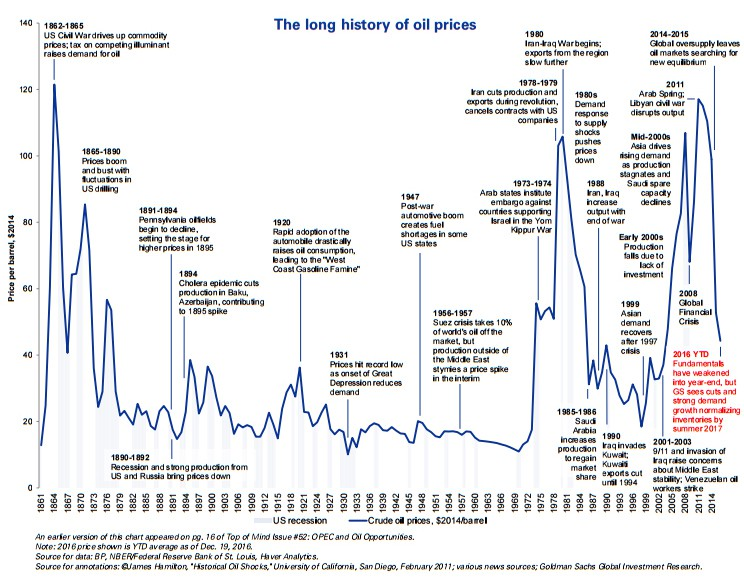
\includegraphics[scale=0.35]{../Figures/Tema_04.01_new.jpg}
\end{frame} 

\begin{frame}
\frametitle{Al precio lo determinan la demanda y la oferta}
\begin{itemize}
    \item Por un lado, tenemos la curva de demanda
    \begin{itemize}
        \item Muestra la cantidad total que los consumidores están dispuestos a comprar a cualquier precio dado
        \item Representa la disposición a pagar (willingness to pay) dinero por los productos que compran
    \end{itemize}
    \vspace{2mm}
    \item Por otro lado, tenemos la curva de oferta
    \begin{itemize}
        \item Muestra la cantidad total que las empresas producirían a cualquier precio dado
        \item Representa la disposición a aceptar (willingness to accept) dinero por los productos que venden
        \item Refleja entonces los distintos precios de reserva de estos vendedores
        \end{itemize}
\end{itemize}
\end{frame}

\begin{frame}
\frametitle{Las curvas se encuentran en un punto}
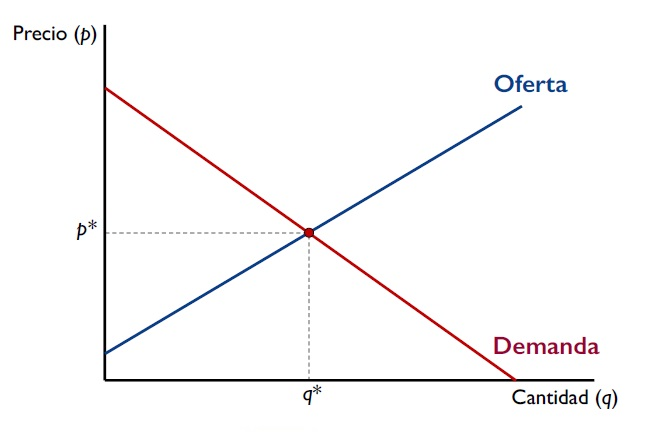
\includegraphics[scale=0.6]{../Figures/Tema_07.3_equilibrioofertademanda_0.jpg}
%Figura 15.1
\end{frame}

\begin{frame}
\frametitle{Equilibrio}
\begin{itemize}
    \item En el precio de equilibrio (market-clearing price), la oferta iguala a la demanda
    \item Otros precios no son un equilibrio de Nash
    \begin{itemize}
        \item Si p $>$ p*, entonces habría exceso de oferta %link que me tire a exceso de oferta (slide siguiente)\\
        - Algunos vendedores desearán vender mayor cantidad pero no encontrarían compradores, podrían beneficiarse de cobrar un precio más bajo
        \item Si p $<$ p*, entonces habría exceso de demanda %link que me tire a exceso de demanda (slide siguiente siguiente) \\
        - Algunos compradores solicitan comprar más cantidad pero no encontrarían vendedores, podrían beneficiarse de cobrar un precio más alto
        \item Se asume que los productos son idénticos, por lo que los compradores estarían dispuestos a comprar a cualquier vendedor
    \end{itemize}
\end{itemize}
\end{frame}

\begin{frame}
\frametitle{Exceso de oferta}
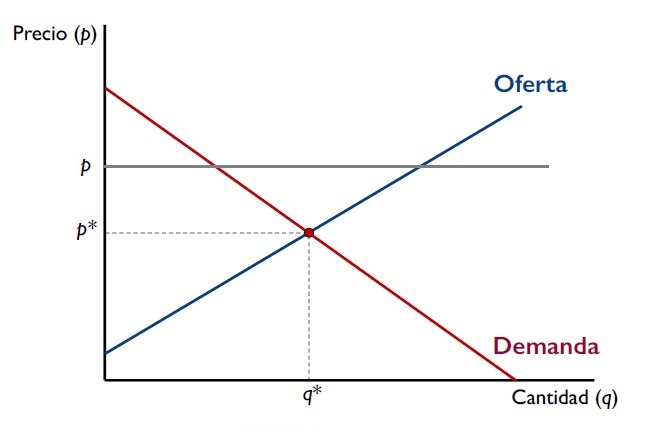
\includegraphics[scale=0.6]{../Figures/Tema_07.3_equilibrioofertademanda_0excesodeoferta.jpg}
%Figura 15.2
\end{frame}

\begin{frame}
\frametitle{Exceso de demanda}
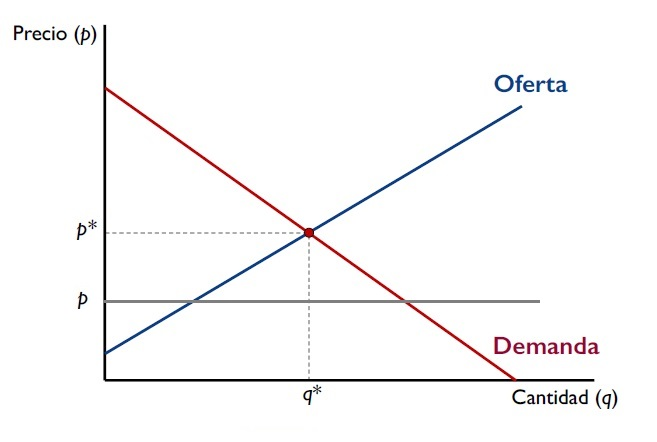
\includegraphics[scale=0.6]{../Figures/Tema_07.3_equilibrioofertademanda_0excesodedemanda.jpg}
%Figura 15.3
\end{frame}

\begin{frame}
\frametitle{Mercados}
\begin{itemize}
    \item Podemos usar todo lo que aprendimos para ver que ocurre en los mercados con los cambios en los precios
\end{itemize}
\end{frame}

\begin{frame}
\frametitle{Ejemplo 1. ¿Qué pasa si aumenta el precio de un bien sustituto?}
\centering
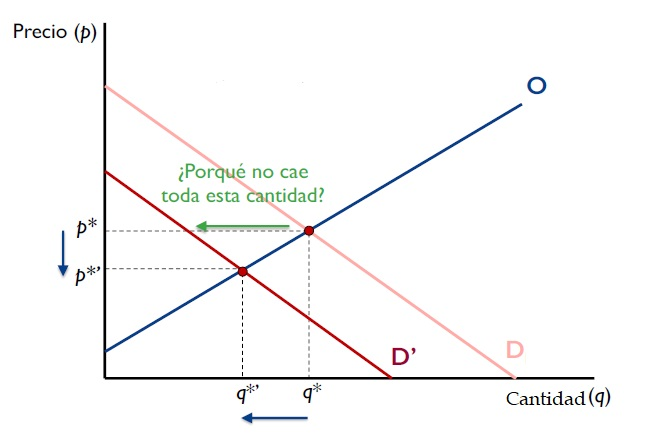
\includegraphics[scale=0.6]{../Figures/Tema_07.4_equilibrioofertademanda.jpg}
% Usar el grafico 15.5 
\end{frame}

\begin{frame}
\frametitle{Ejemplo 2, ¿Qué pasa si aumenta el costo de producir el bien?}
\centering
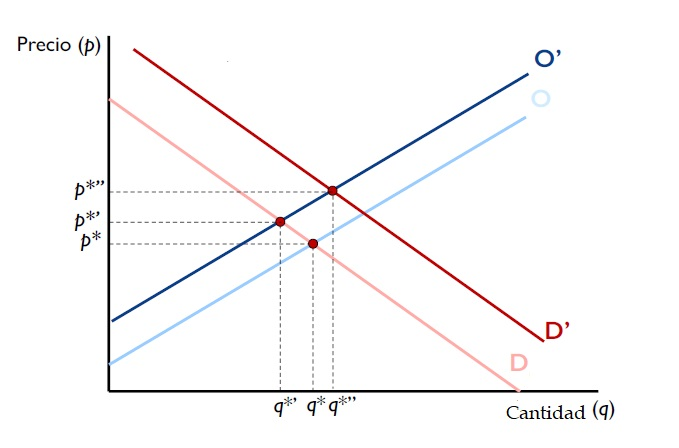
\includegraphics[scale=0.55]{../Figures/Tema_07.5_equilibrioofertademanda2.jpg}
% Grafico 15.6
\end{frame}

% \begin{frame}
% \frametitle{Ejemplo 3: ¿Qué sucede si caen los ingresos de los consumidores y, al mismo tiempo, hay un avance tecnológico?}
% \centering
% \includegraphics[scale=0.6]{../Figures/}
% % Grafico 15.7
% \end{frame}

\begin{frame}
\frametitle{¿Qué desplazamientos de la curvas son consistentes con estos dos puntos?}
\centering
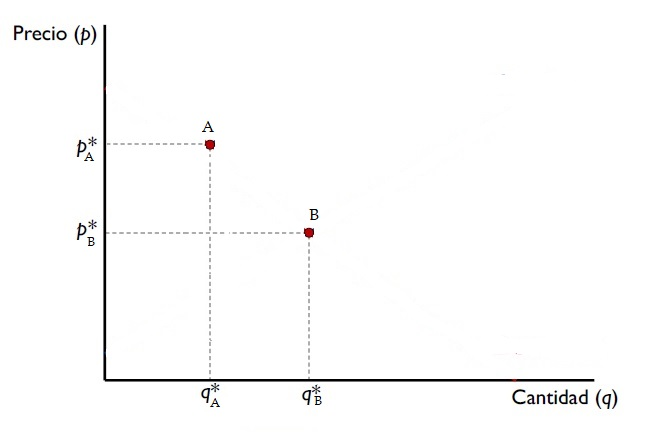
\includegraphics[scale=0.6]{../Figures/Tema_07.6_equilibrioofertademanda3.jpg}
% HACER GRAFICO QUE SEA IGUAL QUE EL LIBRO
\end{frame}


\begin{frame}
\frametitle{Beneficios para todos!}
\begin{itemize}
    \item Los compradores y vendedores comercian en forma voluntaria, ya que ambos se benefician
\end{itemize}
\centering
%\includegraphics[scale=0.5]{Figures/winwin.jp}
\end{frame}

\begin{frame}
\frametitle{Pensando a lo Pareto}
\begin{itemize}
    \item ¿Cuándo una asignación es mejor que otra?
    \begin{itemize}
        \item Una asignación A domina en el sentido de Pareto (Pareto dominates) a otra si al menos alguien está mejor en A y nadie está peor
        \item Si una asignación no está dominada en el sentido de Pareto por ninguna otra, decimos que es eficiente en el sentido de Pareto (Pareto-efficient)
    \end{itemize}
    \item ¡ATENCION! Puede haber más de una asignación Pareto eficiente pero el criterio no nos dice cuál es mejor, y tampoco nos dice nada sobre equidad 
\end{itemize}
\end{frame}

\begin{frame}
\frametitle{¿Cómo medimos las ganancias?}
\begin{itemize}
    \item Podemos medir los beneficios mutuos de una asignación con lo que denominamos 'excedentes' 
    \begin{itemize}
        \item ¿Cuál es la ganancia para el consumidor? \\
        - Cualquier comprador cuya disposición a pagar por un bien sea más alta que el precio de mercado recibe un excedente igual a la diferencia entre esta disposición y el precio pagado
        \item ¿Cuál es la ganancia para el productor? \\
        - Si el costo marginal de producir un bien es inferior al precio de mercado, el productor recibe un excedente
    \end{itemize}
    \end{itemize}
\end{frame}

\begin{frame}
\frametitle{Excedentes}
\begin{itemize}
    \item Las ganancias totales del intercambio están determinadas por los excedentes de consumidores y productores
    \begin{itemize}
        \item El excedente del consumidor \\ - Diferencia entre disposición a pagar y precio de compra
        \item Excedente del productor \\ - Diferencia entre precio y costo de una unidad adicional
    \end{itemize}
    \end{itemize}
\end{frame}

\begin{frame}
\frametitle{Las ganancias del intercambio: la asignación eficiente}
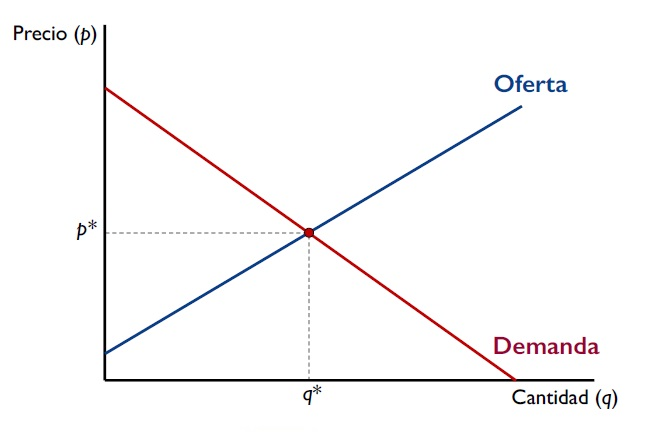
\includegraphics[scale=0.55]{../Figures/Tema_07.3_equilibrioofertademanda_0.jpg}
\end{frame} 

\begin{frame}
\frametitle{Equilibrio y excedentes}
\begin{center}
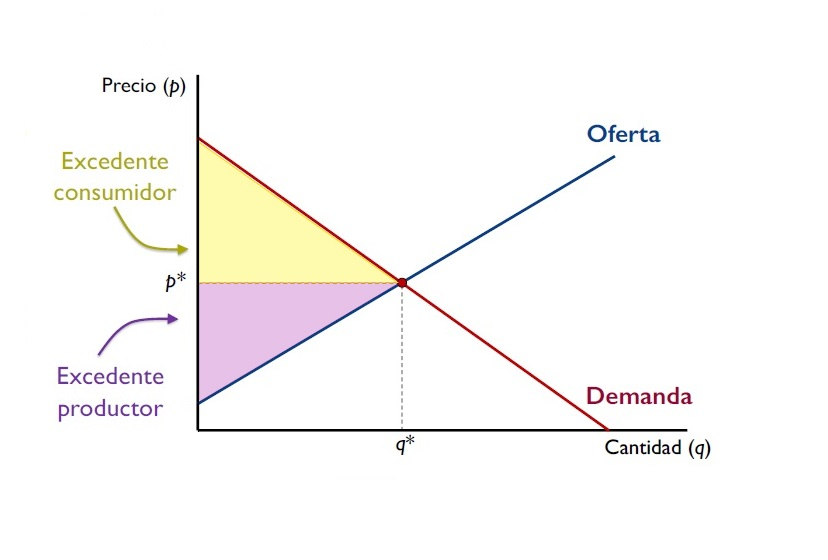
\includegraphics[scale=0.5]{../Figures/Tema_07.23_newexcedentes.jpg}
\end{center}
\end{frame}

\begin{frame}
\frametitle{Pérdida de peso muerto}
\begin{itemize}
    \item ¿Qué pasa si no terminamos en una asignación eficiente? 
    \item Tenemos una ‘pérdida de peso muerto’
    \begin{itemize}
        \item Pérdida de excedente total con respecto a una asignación eficiente \\
        - Es decir, hay ganancias no explotadas del comercio
    \end{itemize}
    \end{itemize}
\end{frame}

\begin{frame}
\frametitle{Precio inicial y excedentes}
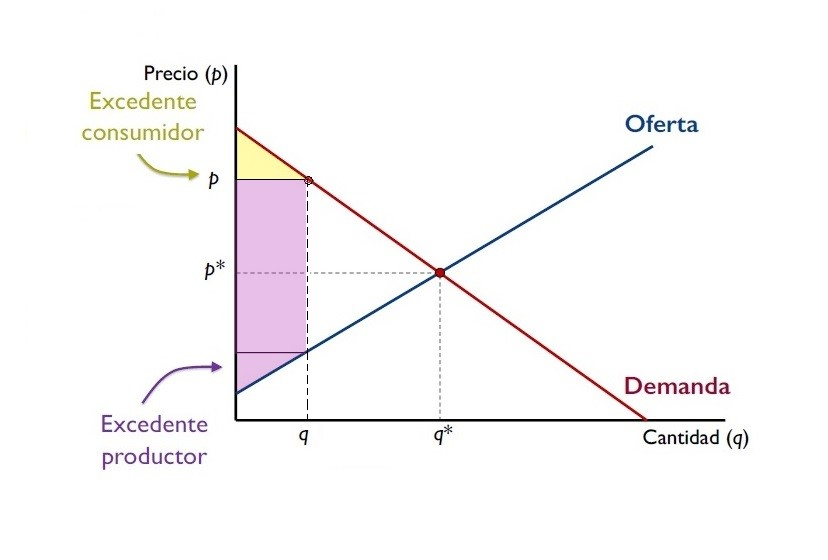
\includegraphics[scale=0.6]{../Figures/Tema_07.23_newexcedentes1.jpg}
\end{frame}

\begin{frame}
\frametitle{Mejora de Pareto}
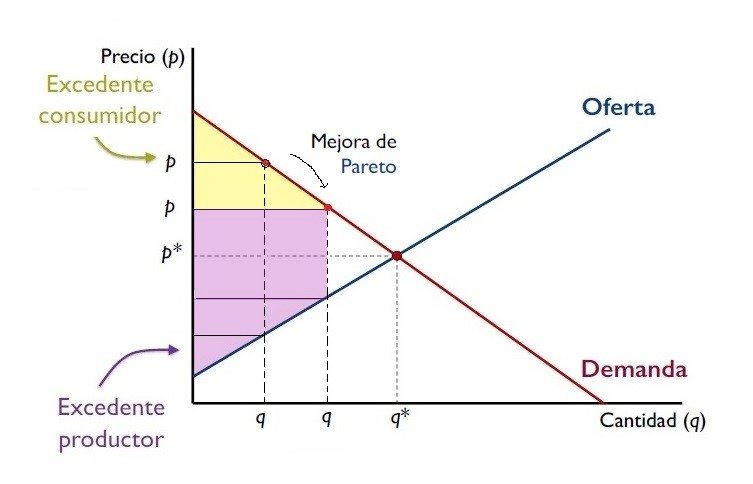
\includegraphics[scale=0.6]{../Figures/Tema_07.23_newexcedentes2.jpg}
\end{frame}

\begin{frame}
\frametitle{Eficiencia de Pareto}
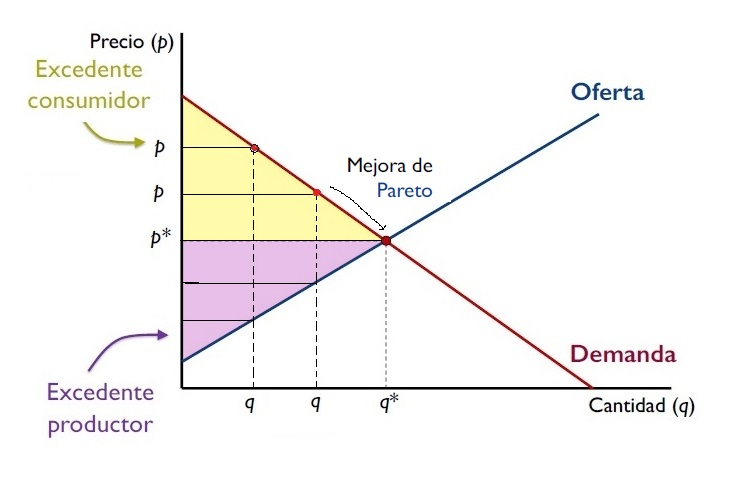
\includegraphics[scale=0.6]{../Figures/Tema_07.23_newexcedentes3.jpg}
\end{frame}

\end{document}


\begin{frame}
\frametitle{Sensibilidad de la demanda}
\begin{itemize}
    \item La pendiente de la curva de demanda tiene información relevante para las empresas
    \begin{itemize}
        \item La pendiente muestra la relación costo-beneficio que la firma enfrenta entre precio y cantidad
     \end{itemize}
    \item ¿Nos ayuda a pensar qué tan sensible es la demanda ante cambios en los precios?
    \begin{itemize}
        \item En parte, si, pero para pensar en esto usamos el concepto de \textbf{elasticidad-precio}: \\
        - Intuitivamente, se refiere al grado de reacción de los consumidores a cambios en el precio del producto 
    \end{itemize}
    \end{itemize}
\end{frame}

\begin{frame}
\frametitle{Elasticidad precio de la demanda}
\begin{itemize}
    \item A diferencia de la pendiente, la elasticidad precio mira cambios porcentuales:
    \begin{center}
    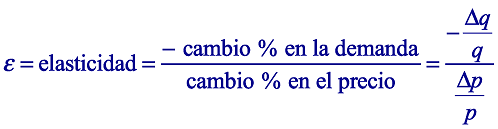
\includegraphics[scale=0.7]{../Figures/Tema_06.43_elasticidadformula.png}
    \end{center}
    \end{itemize}
\end{frame}

\begin{frame}
\frametitle{Elasticidad precio de la demanda}
\begin{itemize}
    \item Medida de sensibilidad: ¿cuál es el cambio \% en la cantidad demandada ante un cambio de 1\% en el precio? \\
    \begin{itemize}
        \item Como la demanda cae ante un aumento en el precio, se suele cambiar el signo para que la relación nos de positiva (esto facilita la interpretación)
    \end{itemize}
    \item ¿Qué tan elástica? \\
    - Si $e > 1$ decimos que la demanda es elástica \\
    - Si $e = 1$ decimos que la demanda es unitaria \\
    - Si $e < 1$ decimos que la demanda es inelástica
    \end{itemize}
\end{frame}

\begin{frame}
\frametitle{Elasticidad y pendiente}
\begin{itemize}
    \item Ambos conceptos están relacionados
    \begin{center}
    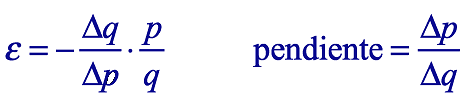
\includegraphics[scale=0.5]{../Figures/Tema_06.44_elasticidadpendiente.png}
    \end{center}
        \begin{itemize}
        \item La pendiente forma parte del concepto de elasticidad
        \item Una curva de demanda muy empinada es relativamente inelástica, y una bastante plana es elástica
        \end{itemize}
    \item ¡Pero no son lo mismo!
        \begin{itemize}
            \item Notar que la elasticidad puede cambiar a medida que nos movemos a lo largo de la curva de demanda, aun si la pendiente no lo hace
            \item ¡Y viceversa!
        \end{itemize}
    \end{itemize}
\end{frame}

\begin{frame}
\frametitle{Elasticidad constante}
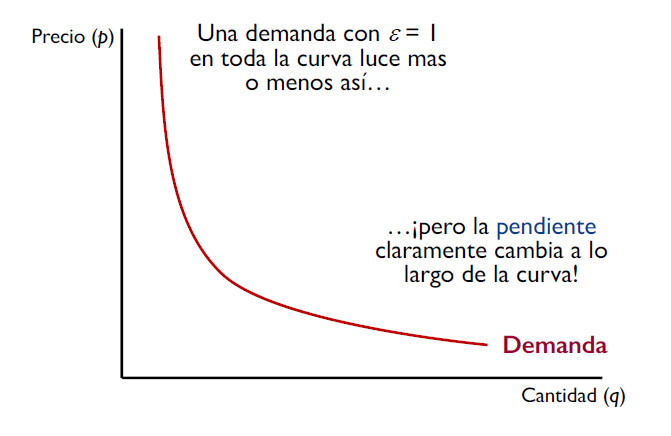
\includegraphics[scale=0.6]{../Figures/Tema_06.45_elasticidad.png}
\end{frame}

\begin{frame}
\frametitle{Pendiente constante}
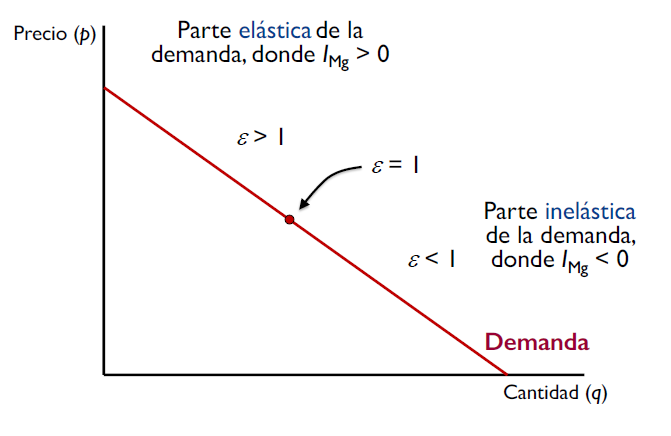
\includegraphics[scale=0.6]{../Figures/Tema_06.46_elasticidad2.png}
\end{frame}

\begin{frame}
\frametitle{¿Cómo son los excedentes con una demanda elástica?}
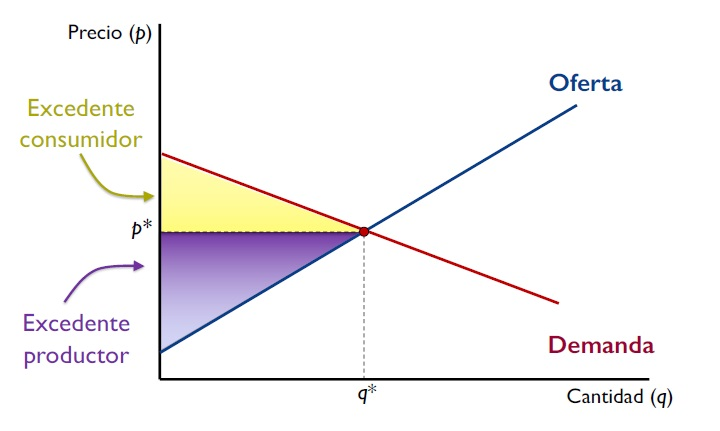
\includegraphics[scale=0.6]{../Figures/Tema_07.24_equilibrioyexcedente2.jpg}
\end{frame}

\begin{frame}
\frametitle{¿Cómo son los excedentes con una demanda inelástica?}
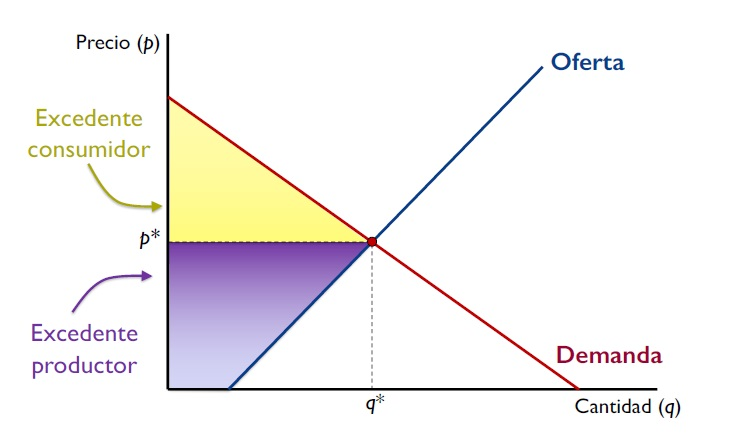
\includegraphics[scale=0.6]{../Figures/Tema_07.25_equilibrioyexcedente3.jpg}
\end{frame}

\begin{frame}
\frametitle{¿Cómo son los excedentes con una oferta elástica?}
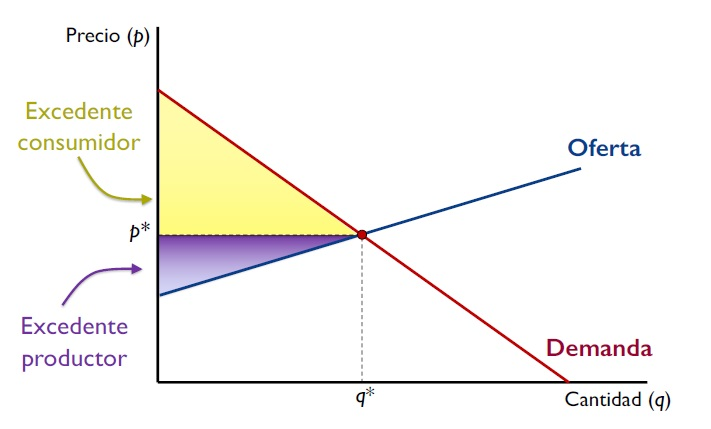
\includegraphics[scale=0.6]{../Figures/Tema_07.26_equilibrioyexcedente4.jpg}
\end{frame}

\begin{frame}
\frametitle{¿Cómo son los excedentes con una oferta inelástica?}
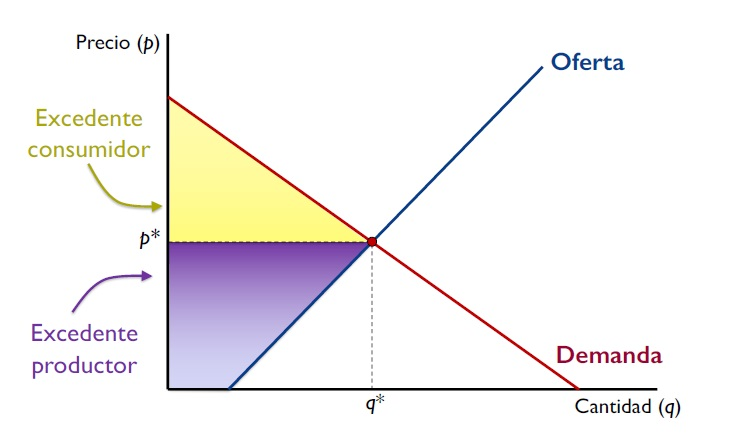
\includegraphics[scale=0.55]{../Figures/Tema_07.25_equilibrioyexcedente3.jpg}
\end{frame}








\begin{frame}
\frametitle{20. ¿Por qué es eficiente?}
\begin{itemize}
    \item Los participantes son tomadores de precios
    \begin{itemize}
        \item No hay poder de mercado
        \item La competencia impide a los vendedores aumentar el precio, y a los compradores bajarlo
    \end{itemize}
    \item Los contratos son completos
        \begin{itemize}
        \item Los detalles del intercambio pueden ser definidos en forma clara, y estos contratos se pueden hacer cumplir
        \end{itemize}
    \item No hay externalidades
        \begin{itemize}
        \item La transacción sólo afecta a los compradores y vendedores
        \end{itemize}
\end{itemize}
\end{frame}


Si llego con el modelo de la telaraña esta bueno para explicarlo

\begin{frame}
\frametitle{3. El precio de la soja}
\centering
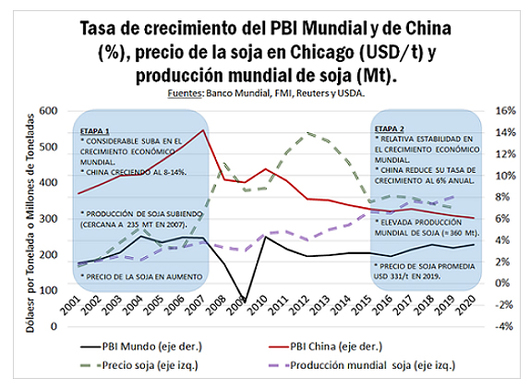
\includegraphics[scale=0.5]{Figures/Tema_04.02_new.jpg}
\end{frame} 


\begin{frame}
\frametitle{41. El impacto de los impuestos}
\begin{itemize}
    \item ¿Qué es un impuesto?
    \begin{itemize}
        \item Es un tributo generalmente establecido por el Estado 
        - para financiar sus gastos
        - para ‘guiar’ el comportamiento (por ejemplo en el caso de externalidades)
    \end{itemize}
    \item Existen diversos tipos:
    \begin{itemize}
        \item Al consumo, al trabajo, al ingreso, a la propiedad, etc.
    \end{itemize}
    \item Un impuesto aumentará el precio que los consumidores pagan sobre un bien...
    \item La elasticidad precio de la demanda tendrá influencia sobre el efecto del impuesto
\end{itemize}
\end{frame}

\begin{frame}
\frametitle{42. Impuestos y eficiencia}
\begin{itemize}
    \item La introducción de impuestos aleja la economía del equilibrio competitivo
    \begin{itemize}
        \item Los impuestos sobre oferentes/consumidores desplazan la curva de oferta/demanda porque el precio es más alto para cada cantidad
        \item Al recaudar impuestos el Estado genera una pérdida de peso muerto
    \end{itemize}
    \item La recaudación se extrae del excedente de consumidores y productores
    \begin{itemize}
        \item La incidencia del impuesto depende de la elasticidad relativa de consumidores y productores
        \item El grupo menos elástico lleva más de la carga fiscal
    \end{itemize}
\end{itemize}
\end{frame}

\begin{frame}
\frametitle{43. Impacto de un impuesto a los vendedores}
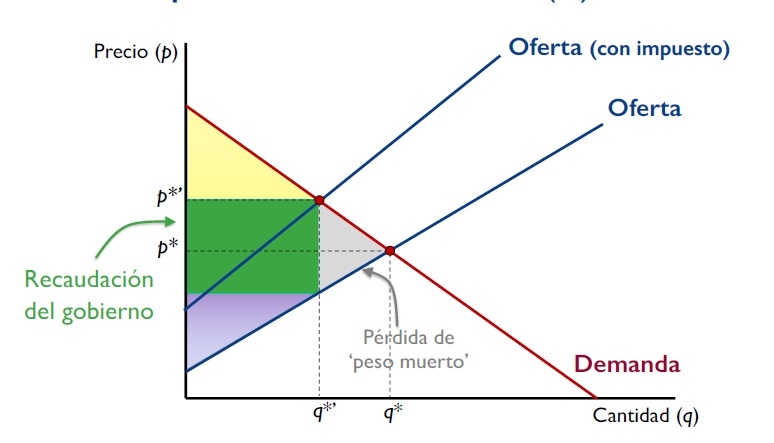
\includegraphics[scale=0.6]{Figures/Tema_07.29_impuesto1.jpg}
\end{frame}

\begin{frame}
\frametitle{44. Impacto de un impuesto a los vendedores}
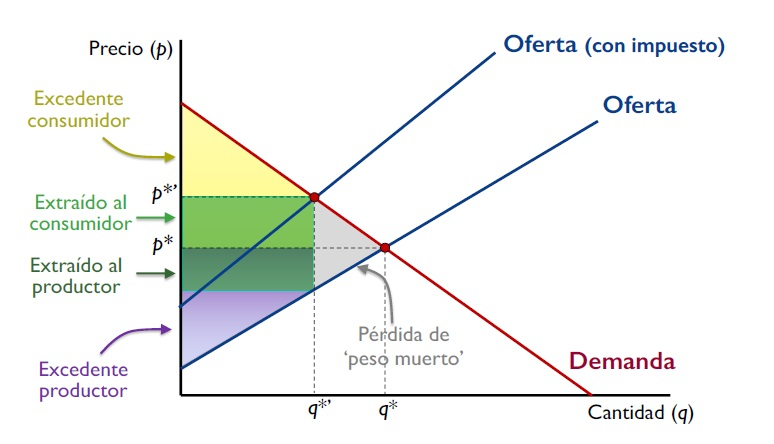
\includegraphics[scale=0.6]{Figures/Tema_07.30_impuesto2.jpg}
\end{frame}

\begin{frame}
\frametitle{45. Impacto de los impuestos}
\begin{itemize}
    \item ¿Cuánto va a cambiar los impuestos el comportamiento de los individuos?
    \begin{itemize}
        \item ¿Qué tan grande va a ser la pérdida de peso muerto? \\
        - ¿Porqué es relevante conocer la elasticidad de demanda? \\
        - ¿Qué tipo de productos tienen demanda inelástica?
    \end{itemize}
    \item ¿Qué hace el gobierno con los recursos que recauda?
    \item A veces el gobierno quiere cambiar el comportamiento
\end{itemize}
\end{frame}

\begin{frame}
\frametitle{46. Impuestos y elasticidad}
\begin{itemize}
    \item Un impuesto puede reducir mucho las ventas si su demanda es altamente elástica
    \begin{itemize}
        \item ¡Y eso puede ser lo que el gobierno intenta hacer! \\
        - P.ej., impuestos sobre bienes ‘malos’ para la sociedad como el tabaco o el alcohol o por contaminar
    \end{itemize}
    \item Pero si un impuesto causa una importante caída en las ventas, también reduce los ingresos del impuesto
    \item Si un gobierno que desea aumentar los ingresos a partir del impuesto, debería elegir gravar productos con demanda inelástica
    \begin{itemize}
        \item ¿Qué tipo de productos pueden tener una demanda de estas características?
    \end{itemize}
\end{itemize}
\end{frame}